% !TEX root = main.tex

\section{Balancing Data Sets}
\label{sec:balance}

As mentioned previously, Dex-Net 2.0 contains approximately 20\% positive examples. 
Na{\"i}vely, you could predict a negative label for all instances and be correct 80\% of the time. Interesting, the paper reported an 85.7\% accuracy, which does slightly better than an all negative classifier. 

To investigate this, we begin by using the \rhnote{pretrained dex net network} on the data sets we created by sampling the entire Dex Net data base. 
We can constrain our sampling to produce a data set of 10,000 samples that is 50\% positive examples and 50\% negative examples (referred to as a "balanced" data set). 
Using their network we achieve approximately 50\% accuracy because, as shown in our confusion matrix in \figref{fig:balanced_confusion}, the network learns to always output a positive label. 

If we do not make such a constraint and sample randomly, we expect to have the original distribution: 20\% positive examples and 80\% negative examples (referred to as an "unbalanced" data set). 
As shown by the confusion matrix in \figref{fig:unbalanced_confusion}, the network achieved approximately 80\% accuracy by always guessing negative. 

To confirm our thoughts a step further, we use the data they provide on the network they provide (\rhnote{confirm}). 
This data set is also unbalanced and achieves similarly to above in that it always guesses negative, as seen in \figref{fig:from_paper}. 

This result was initially surprising. 
Due to the few percentage point disparity between our accuracy and theirs, we hesitate to conclusively claim their network did not learn features. 
While we varied the size of the data set we use, we did not come close to their magnitude (in the millions) and therefore it is possible that the network simply needs a tremendous amount of data to learn effectively. 

To explore further, we experiment with varying the architecture of the CNN. 
This both allows us to explore the effect of the architecture (as well as its hyper-parameters) and to see if we can improve upon our accuracy rate. 

\begin{figure*}[t!]
    \begin{subfigure}[t]{0.24\textwidth}
        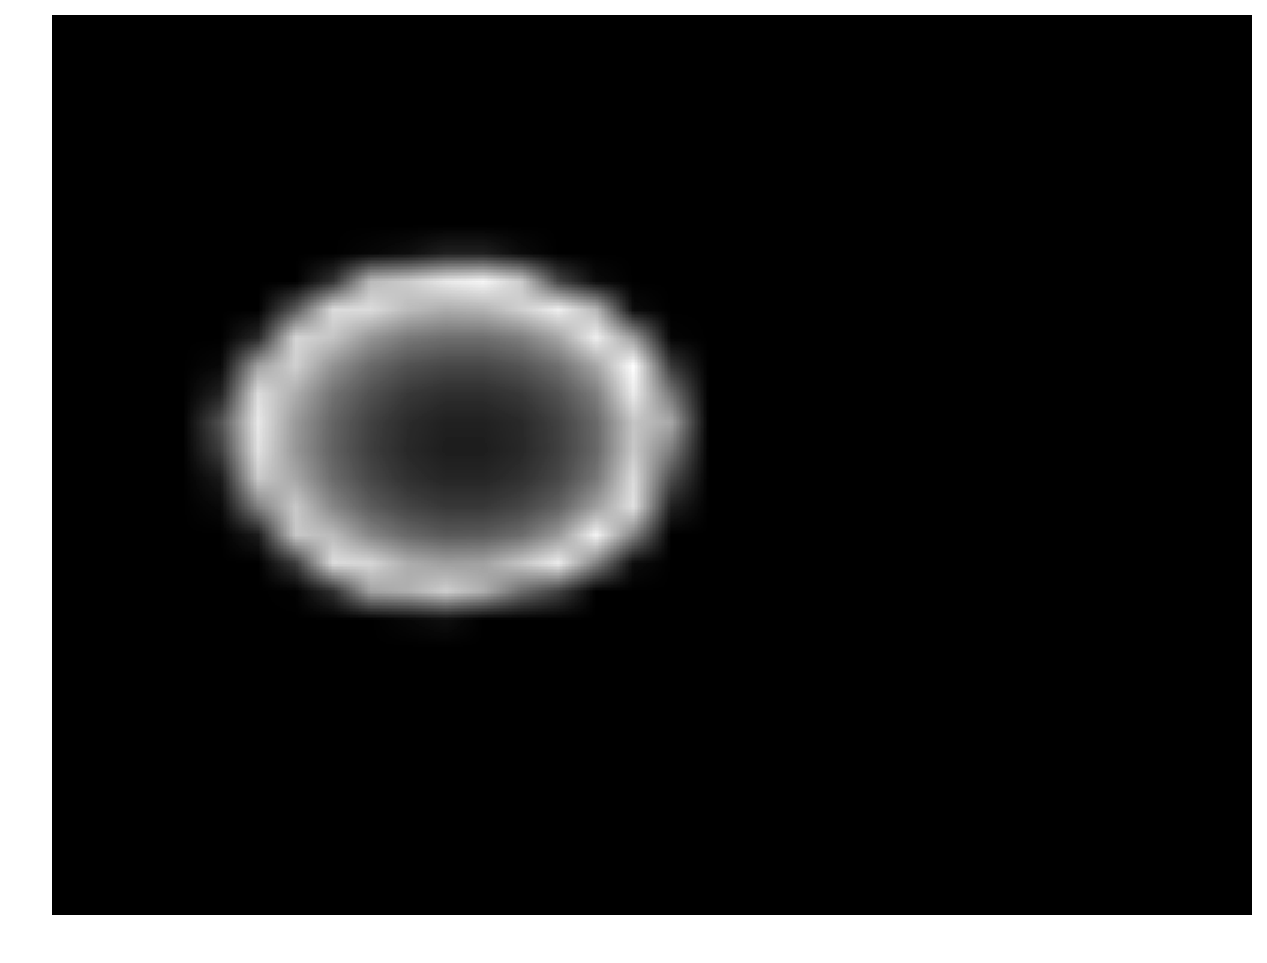
\includegraphics[width=0.75\columnwidth]{figs/depth_example.pdf} \caption{Example Depth Image} \label{fig:depth_image}
        \end{subfigure}
    \begin{subfigure}[t]{0.24\textwidth}
        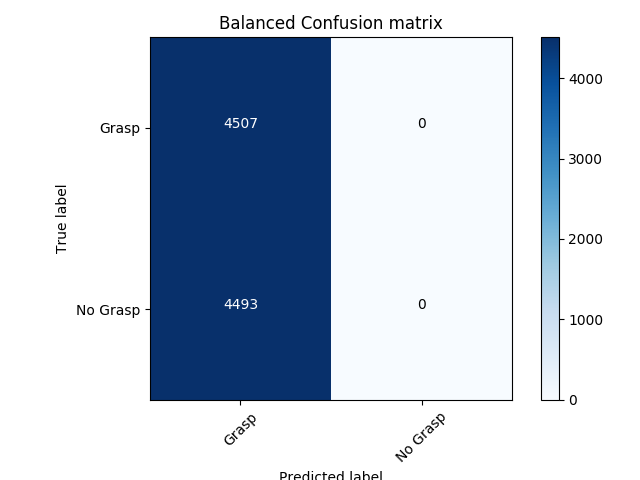
\includegraphics[width=0.9\columnwidth]{figs/balanced_results.png} \caption{Balanced Data} \label{fig:balanced_confusion}
    \end{subfigure}
		\begin{subfigure}[t]{0.24\textwidth}
        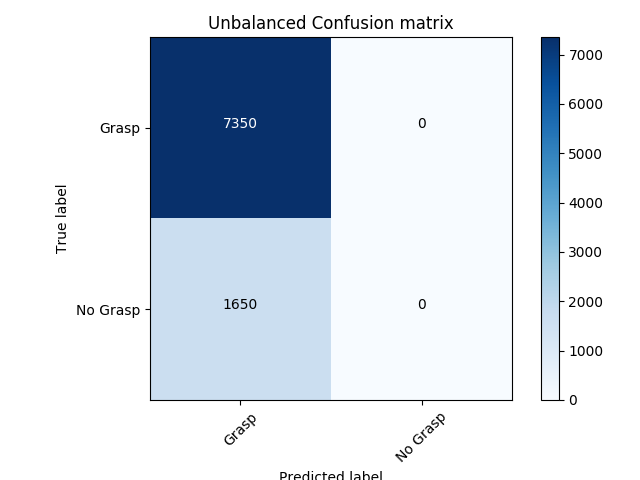
\includegraphics[width=0.9\columnwidth]{figs/unbalanced_results.png} \caption{Unbalanced Data} \label{fig:unbalanced_confusion}
        \end{subfigure}
    \begin{subfigure}[t]{0.24\textwidth}
        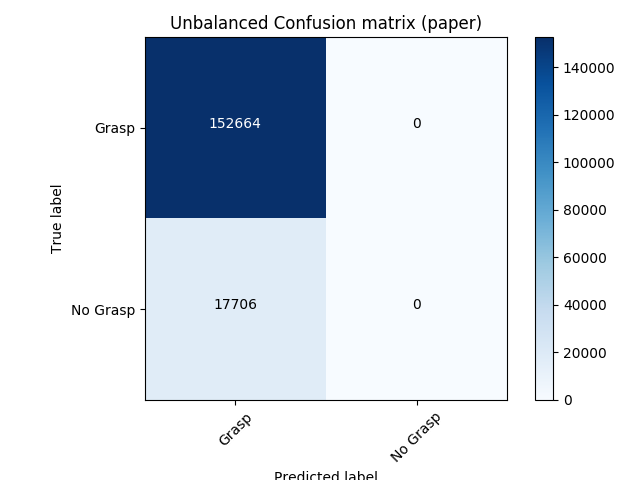
\includegraphics[width=0.9\columnwidth]{figs/paper_original.png} \caption{Replicated Paper Results} \label{fig:from_paper}
    \end{subfigure}
\caption{FILL IN CAPTION} \label{fig:confusion_matrices}
\end{figure*}